%%%%%%%%%%%%%%%%%%%%%%%%%%%%%%%%%%%%%%%%%%%%%%%%%%%%%%%%%%%%%%%%%%%%%%%%%
%%%% Plantilla realizada por César Martínez cesar.martinez@udlap.mx %%%%%
%%%%%%%%%%%%%%%%%%%%%%%%%%%%VERSION 1.0%%%%%%%%%%%%%%%%%%%%%%%%%%%%%%%%%%
%%%%%%%%%%%%%%%%%%%%%%%%%%%%%%%%%%%%%%%%%%%%%%%%%%%%%%%%%%%%%%%%%%%%%%%%%
%%%%%%%%%%%%%%%%%%%%%%%%%%%%%%%%%%%%%%%%%%%%%%%%%%%%%%%%%%%%%%%%%%%%%%%%%


\documentclass[12pt]{article}  %tipo de documento y tamaño de letra normal
%%%%%%%%%%%%%%%%%%%%%%%%%%%%%%%%%%%%%%%%%%%%%%%%%%%%%%%%%%%%%%%%%%%%%
%%%%%%%%%%%%%%%%%%%%%%%%%%%%%%%%%%%%%%%%%%%%%%%%%%%%%%%%%%%%%%%%%%%%%
%%%%%%%%%%%%%%%%%%%%%%%%%%%%%%%%%%%%%%%%%%%%%%%%%%%%%%%%%%%%%%%%%%%%%
%%%%%%%% Paquetes basicos, pueden encontrar información especifica de cada uno de ellos en  (https://www.ctan.org/) %%%%%%%%%%%%%%%%%%%%%%% %%%%%%%%%%%%%%%%%%%%%%%%%%%%%%%%%%%%%%%%%%%%%%%%%%%%%%%%%%%%%%%%%%%%%
%%%%%%%%%%%%%%%%%%%%%%%%%%%%%%%%%%%%%%%%%%%%%%%%%%%%%%%%%%%%%%%%%%%%%
%%%%%%%%%%%%%%%%%%%%%%%%%%%%%%%%%%%%%%%%%%%%%%%%%%%%%%%%%%%%%%%%%%%%%
%\usepackage[spanish]{babel} %Indica que escribiermos en español
\usepackage[english]{babel} %Indica que escribiermos en inglés
%Comentar la línea del idioma que NO usarán en su reporte
\usepackage[utf8]{inputenc} %Indica qué codificación se está usando ISO-8859-1(latin1)  o utf8  
\usepackage{amsmath} % Comandos extras para matemáticas (cajas para ecuaciones,etc)
\usepackage{amssymb} % Simbolos matematicos (por lo tanto)
\usepackage{graphicx} % Incluir imágenes en LaTeX
\usepackage{color} % Para colorear texto
\usepackage{subfigure} % subfiguras
\usepackage{enumerate} % enumerar
\usepackage{commath} % funcionalidades extras para diferenciales, integrales,etc (\od, \dif, etc)
\usepackage{cancel} % para cancelar expresiones (\cancelto{0}{x})
\usepackage{float} %Podemos usar el especificador [H] en las figuras para que se queden donde queramos
\usepackage{appendix} %Para crear apendices
\usepackage{xcolor} %Definir colores personalizados
%%%%%%%%%%%%%%%%%%%%%%%%%%%%%%%%%%%%%%%%%%%%%%%%%%%%%%%%%%%%%%%%%%%%%
%%%%%%%%% PAQUETES CON OPCIONES ESPECIFICAS PRECARGADAS %%%%%%%%%%%%%
%%%%%%%%%%%%%%%%%%%%%%%%%%%%%%%%%%%%%%%%%%%%%%%%%%%%%%%%%%%%%%%%%%%%%
%%%%%%%%%%%%% Permitir agregar código, colocarlo en un rectángulo y  numerarlo %%%%%%%%%%%%%%%%%%%%%%%%%%%%%%%%%%%%%%%%%%%%%%%%%%%%%%%%%%%
%%%%%%%%%%%%%%%%%%%%%%%%%%%%%%%%%%%%%%%%%%%%%%%%%%%%%%%%%%%%%%%%%%%%%
%%%%%%%%%%%%%%%%%%%%%%%%%%%%%%%%%%%%%%%%%%%%%%%%%%%%%%%%%%%%%%%%%%%%%%%%%%%%%%%%%%%%%%%%%%%%%%%%%%%%%%%%%%%%%%%%%%%%%%%%%%%%%%%%%%%%%%%%%%
\usepackage{listings} %Sirve para pegar codigo fuente de programas
\usepackage{caption} %Agregar titulos a los codigos
\DeclareCaptionFont{white}{\color{white}}
\DeclareCaptionFormat{listing}{%
  \parbox{\textwidth}{\colorbox{gray}{\parbox{\textwidth}{#1#2#3}}\vskip-4pt}}
\captionsetup[lstlisting]{format=listing,labelfont=white,textfont=white}
\lstset{frame=lrb,xleftmargin=\fboxsep,xrightmargin=-\fboxsep}
\renewcommand{\lstlistingname}{Código}
%%%%%%%%%%%%%%%%%%%%%%%%%%%%%%%%%%%%%%%%%%%%%%%%%%%%%%%%%%%%%%%%%%%%%
%%% Definir márgenes del documento%%%%%%%%%%%%%%%%%%%%%%%%%%%%%%%%%%%
%%%%%%%%%%%%%%%%%%%%%%%%%%%%%%%%%%%%%%%%%%%%%%%%%%%%%%%%%%%%%%%%%%%%%
 \usepackage{anysize} % Para personalizar el ancho de  los márgenes
\marginsize{2cm}{2cm}{2cm}{2cm} % Izquierda, derecha, arriba, abajo
%%%%%%%%%%%%%%%%%%%%%%%%%%%%%%%%%%%%%%%%%%%%%%%%%%%%%%%%%%%%%%%%%%%%
%%% Hipervinculos activos y a color %%%%%%%%%%%%%%%%%%%%%%%%%%%%%%%%
%%%%%%%%%%%%%%%%%%%%%%%%%%%%%%%%%%%%%%%%%%%%%%%%%%%%%%%%%%%%%%%%%%%%%
\usepackage[colorlinks=true,plainpages=true,citecolor=blue,linkcolor=black]{hyperref}
\usepackage{hyperref} 
%%%%%%%%%%%%%%%%%%%%%%%%%%%%%%%%%%%%%%%%%%%%%%%%%%%%%%%%%%%%%%%%%%%%%
%%%%%% Encabezado y pie de pagina %%%%%%%%%%%%%%%%%%%%%%%%%%%%%%%%%%%
%%%%%%%%%%%%%%%%%%%%%%%%%%%%%%%%%%%%%%%%%%%%%%%%%%%%%%%%%%%%%%%%%%%%%
\usepackage{fancyhdr} 
\pagestyle{fancy}
\fancyhf{}
\fancyhead[L]{\footnotesize UDLAP} %encabezado izquierda
\fancyhead[R]{\footnotesize CEM}   % encabezado derecha
\fancyfoot[R]{\footnotesize \curso}  % Pie derecha
\fancyfoot[C]{\thepage}  % centro
\fancyfoot[L]{}  %izquierda
\renewcommand{\footrulewidth}{0.4pt}
%%%%%%%%%%%%%%%%%%%%%%%%%%%%%%%%%%%%%%%%%%%%%%%%%%%%%%%%%%%%%%%%%%%%%
%%%% Carpeta donde se deben colocar las imagenes %%%%%%%%%%%%%%%%%%%%
\graphicspath{{Imagenes/}} %Colocar aqui todas las imagenes del documento pueden estar en formato png, eps o jpg, se recomienda eps para mayor calidad.
%%%%%%%%%%%%%%%%%%%%%%%%%%%%%%%%%%%%%%%%%%%%%%%%%%%%%%%%%%%%%%%%%%%%%
%%%%%%%%%%%%%%%%%%%%%%%%%%%%%%%%%%%%%%%%%%%%%%%%%%%%%%%%%%%%%%%%%%%%%
%%%%%%%% Termina carga de paquetes %%%%%%%%%%%%%%%%%%%%%%%%%%%%%%%%%%% 
%%%%%%%%%%%%%%%%%%%%%%%%%%%%%%%%%%%%%%%%%%%%%%%%%%%%%%%%%%%%%%%%%%%%%
%%%%%%%%%%%%%%%%%%%%%%%%%%%%%%%%%%%%%%%%%%%%%%%%%%%%%%%%%%%%%%%%%%%%%
%%%%%%%%%%%%%%%%%%%%%%%%%%%%%%%%%%%%%%%%%%%%%%%%%%%%%%%%%%%%%%%%%%%%%
%%%%%% Modificar campos que aparecerán en portada %%%%%%%%%%%%%%%%%%%
%%%%%%%%%%%%%%%%%%%%%%%%%%%%%%%%%%%%%%%%%%%%%%%%%%%%%%%%%%%%%%%%%%%%%
%%%%%%%%%%%%%%%%%%%%%%%%%%%%%%%%%%%%%%%%%%%%%%%%%%%%%%%%%%%%%%%%%%%%%
%%%%%%%%%%%%%%%%%%%%%%%%%%%%%%%%%%%%%%%%%%%%%%%%%%%%%%%%%%%%%%%%%%%%%
\def\titulo{Lab report \#2}%titulo del documento
\def\materia{Course: Digital design LRT2022-7} %Clave nombre de la materia y sección
\def\curso{Digital design} %Nombre de la materia para footnote
\def\fecha{April 1st, 20} %En formato mes, dia año
\def\equipo {2}%Verificar en blackboard el número asignado
\def\ida{183339} %Nombre y Id´s de todos los integrantes que hayan trabajado en el proyecto
\def\esta{Juan Pablo Lopez Moreno}
\def\lica{LMT}%LRT,LBM,LIS,LMT
\def\idb{185406}
\def\estb{Amy Marianee Ramírez Sánchez}
\def\licb{LMT}%LRT,LBM,LIS,LMT
%Copiar y pegar más líneas si su equipo tiene más de 5 integrantes, eliminar si está formado por menos
%%%%%%%%%%%%%%%%%%%%%%%%%%%%%%%%%%%%%%%%%%%%%%%%%%%%%%%%%%%%%%%%%%%%%
%%%%%%%%%%%%%%%%%%%%%%%%%%%%%%%%%%%%%%%%%%%%%%%%%%%%%%%%%%%%%%%%%%%%%
%%%%%%%%%%%%%%%%%%%%%%%%%%%%%%%%%%%%%%%%%%%%%%%%%%%%%%%%%%%%%%%%%%%%%
\begin{document} %Inicia el documento
%%%%%%%%%%%%%%%%%%%%%%%%%%%%%%%%%%%%%%%%%%%%%%%%%%%%%%%%%%%%%%%%%%%%%
%%%%%%%%%%%%%%%%%%%%%%%%%%%%%%%%%%%%%%%%%%%%%%%%%%%%%%%%%%%%%%%%%%%%%
%%%%%%%%%%%%%%%%%%%%%%%%%%%%%%%%%%%%%%%%%%%%%%%%%%%%%%%%%%%%%%%%%%%%%
%%%%%%%%%%%%%%%%%%%%%%%%%%%%%%%%%% PORTADA %%%%%%%%%%%%%%%%%%%%%%%%%%
%%%%%%%%%%%%%%%%%%%%%%%%%%%%%%%%%%%%%%%%%%%%%%%%%%%%%%%%%%%%%%%%%%%%%No es necesario modificar ninguna de las siguientes lineas, sólo si el número de estudiantes que conforman su equipo es menor o mayor a 5
%%%%%%%%%%%%%%%%%%%%%%%%%%%%%%%%%%%%%%%%%%%%%%%%%%%%%%%%%%%%%%%%%%%%%
%%%%%%%%%%%%%%%%%%%%%%%%%%%%%%%%%%%%%%%%%%%%%%%%%%%%%%%%%%%%%%%%%%%%%
%%%%%%%%%%%%%%%%%%%%%%%%%%%%%%%%%%%%%%%%%%%%%%%%%%%%%%%%%%%%%%%%%%%%%
\begin{center}														
\newcommand{\HRule}{\rule{\linewidth}{0.5mm}}						
\thispagestyle{empty} 												
\vspace*{-1.5cm}								
\textsc{\huge Universidad de las Américas Puebla}\\[1.5cm]	
\textsc{\LARGE Escuela de ingeniería}\\[1.5cm]	
\textsc{\LARGE Departamento de computación, electrónica y mecatrónica}\\[1.5cm]												
\includegraphics[width=150mm]{UDLAP}  									\vspace*{1cm}														\HRule \\[0.4cm]												
{ \huge \bfseries \titulo}\\[0.4cm]	
\HRule \\[1cm]														
{ \Large \bfseries \materia}\\[1cm] 	
{ \Large \bfseries Equipo: \equipo}\\[1cm] 							
\begin{flushleft} \Large											
\ida \hspace{0.5cm}\esta \hspace{0.5cm} \lica\\
\idb \hspace{0.5cm}\estb \hspace{0.5cm} \licb\\
%Copiar y pegar más líneas si su equipo tiene más de 2 integrantes, eliminar si la entrega es individual
\end{flushleft}														
\vfill																
\begin{center}													
{\Large  \fecha, San Andrés Cholula, Puebla}						
\end{center}												 		
\end{center}							 								\newpage						
%%%%%%%%%%%%%%%%%%%% TERMINA PORTADA %%%%%%%%%%%%%%%%%%%%%%%%%%%%%%%%
%%%%%%%%%%%%%%%%%%%%%%%%%%%%%%%%%%%%%%%%%%%%%%%%%%%%%%%%%%%%%%%%%%%%%
%%%%%%%%%%%%%%%%%%%%%%%%%%%%%%%%%%%%%%%%%%%%%%%%%%%%%%%%%%%%%%%%%%%%%
%%%%%%%%%%%%%%%%%%%%%%%%%%%%%%%%%%%%%%%%%%%%%%%%%%%%%%%%%%%%%%%%%%%%%
%%%%%%%%%%%%%%%%%%%%%%%%%%%%%%%%%%%%%%%%%%%%%%%%%%%%%%%%%%%%%%%%%%%%%
\setcounter{page}{1} %Para comenzar a numerar las páginas desde este punto
\section{Abstract} %Síntesis del reporte en un solo párrafo
This report will present the results obtained from the second laboratory practice of the Digital Design course. The main objective of this practice was to familiarize ourselves with the
functioning of logic gates and boolean functions. Showcasing both a physical and simulation function based on logic gates.
\section{Introduction} %Breve introducción al tema del reporte
Logic gates are the fundamental building blocks of digital electronics, as they allow the processing of binary signals through basic logical operations such as AND, OR, and NOT. A logic gate is a device that receives one or more binary input signals (0 or 1) and produces a binary output depending on the logical operation it performs. These operations enable the structured and predictable manipulation of digital information.
There are several types of logic gates, among the most common are:
\begin{itemize}
  \item AND, which outputs 1 only when all its inputs are 1.
  \item OR, which outputs 1 if at least one of its inputs is 1.
  \item NOT, which inverts the value of its input, turning 0 into 1 and vice versa.
  \item Additionally, there are combinations such as NAND, NOR, XOR, and XNOR, which are used to construct more complex functions and optimize circuits.
\end{itemize}\cite{UNAMCompuertas}
From these operations, it is possible to build more complex Boolean functions, representing relationships between binary variables using logical connectors, forming the foundation of digital system design. These functions are essential for developing integrated circuits, microprocessors, memory devices, and modern electronic systems.
In this context, the main objectives of this lab were to implement and verify the operation of basic logic gates, obtain the truth table and canonical form of a Boolean function, and simulate and program digital circuits using VHDL.
In this way, the lab not only aims to experimentally verify the theoretical principles of Boolean algebra but also to develop skills in using simulation software and hardware description languages, which are essential tools in modern digital system design.

\section{Objectives} %Objetivos de la práctica
The objectives of this lab are:
\begin{itemize}
  \item Implement basic circuits to verify the operation of three basic logic gates.
  \item Verify the proper functioning of the digital circuits by using the Multimeter.
  \item Program and simulate basic digital circuits using VHDL
  \item Obtain truth table and canonic form of a Boolean function.
  \item Program and simulate Boolean functions using VHDL.
\end{itemize}
For the purpose of this lab, it is important to know about the components used, in the first place, "logic gates are defined as simple digital circuits that take one or more binary inputs and produce a binary output"\cite{HARRIS20221}.
On the other hand, boolean funtions consists of a number of Boolean variables joined by the Boolean connectives, like AND and OR. \cite{HOLDSWORTH200228}
And last, but not least, the software utilized in the experiment is VHDL (Hardware Description Language), which is a language that describes the behavior of electronic circuits, most commonly digital circuits. \cite{IntelVHDLDef}
\section{Methodology}
A methodology was established, divided into three main phases: physical
implementation in the laboratory, simulation in Multisim, and programming in
EDA Playground.

\subsection{Physical Laboratory Phase}
In the physical laboratory, the following procedure was carried out:
\begin{itemize}
    \item The power supply was configured with the following parameters:
    \begin{itemize}
        \item Activated source: Source 3.
        \item Output voltage: 5 V.
        \item Output current: 300 mA.
    \end{itemize}
    \item Using the datasheets, the power terminals, inputs, and outputs of each logic gate were identified.
    \item The basic circuit of each logic gate was built.
    \item The truth table presented in the datasheet was verified and compared with the one obtained from the real circuit.
    \item The truth table and the canonical form of the Boolean function were obtained:
    $$
    F(A,B,C,D) = (\bar{B} \cdot D) + (\bar{A} \cdot B \cdot \bar{C}) + (A \cdot \bar{B} \cdot C) + (A \cdot B \cdot \bar{C})
    $$
    \item The circuit corresponding to the Boolean function was built.
    \item The truth table of the Boolean function was verified against the one obtained experimentally from the real circuit.
\end{itemize}

\subsection{Multisim Simulation Phase}
In the Multisim environment, the following tasks were performed:
\begin{itemize}
    \item The circuits corresponding to the basic logic gates (AND, OR, XOR, NOT, NAND, NOR, and XNOR) were constructed, simulated, and their correct operation was verified.
    \item The Boolean function defined in point 5 of the laboratory phase was constructed and simulated, confirming its proper functioning.
\end{itemize}

\subsection{EDA Playground Programming Phase}
Finally, in the EDA Playground platform, the following steps were carried
out:
\begin{itemize}
    \item A single file was created to program and verify the correct operation of the basic logic gates (AND, OR, XOR, NOT, NAND, NOR, and XNOR).
    \item The Boolean function F(ABCD) was programmed and simulated.
\end{itemize}

Finally, an analysis was carried out between the results obtained in the simulation and those obtained experimentally in the laboratory.


\section{Results} %Resultados obtenidos
\subsection{Physical lab experimentation}
For the physical lab, the team developed the basic circuits for each logic gate, obtaining the following tables:
\begin{table}[h!]
\centering
\begin{tabular}{|c|c|c|}
\hline
\multicolumn{2}{|c|}{\textbf{Input}} & \textbf{Output} \\
\hline
\textbf{A} & \textbf{B} & \textbf{Y} \\
\hline
0 & 0 & 0 \\
0 & 1 & 0 \\
1 & 0 & 0 \\
1 & 1 & 1 \\
\hline
\end{tabular}
\caption{Truth Table for a 2-Input AND Gate, the 74HC08 integrated circuit.}
\label{tab:and_gate}
\end{table}

\begin{table}[h!]
\centering
\begin{tabular}{|c|c||c|}
\hline
\multicolumn{2}{|c|}{\textbf{Input}} & \textbf{Output} \\
\hline
\textbf{A} & \textbf{B} & \textbf{Y} \\
\hline
0 & 0 & 0 \\
0 & 1 & 1 \\
1 & 0 & 1 \\
1 & 1 & 1 \\
\hline
\end{tabular}
\caption{Truth Table for a 2-Input OR Gate, the 74HC32 integrated circuit.}
\label{tab:or_gate}
\end{table}

\begin{table}[h!]
\centering
\begin{tabular}{|c|c|}
\hline
\textbf{Input} & \textbf{Output} \\
\hline
\textbf{A} & \textbf{Y} \\
\hline
0 & 1  \\
1 & 0  \\
\hline
\end{tabular}
\caption{Truth Table for a 1-Input NOT Gate, the 74HC04 integrated circuit.}
\label{tab:and_gate}
\end{table}

After ensuring that the truth tables were consistent with the datasheets obtained in the pre-lab, the team started analysing the following boolean function:
$$
F(A, B, C, D) = (\bar{B} \cdot D) + (\bar{A} \cdot B \cdot \bar{C}) + (A \cdot \bar{B} \cdot C) + (A \cdot B \cdot \bar{C})
$$ \\
And after analysing the function, the following truth table was formulated:
\begin{table}[h!]
\centering
\begin{tabular}{|c|c|c|c||c|}
\hline
\multicolumn{4}{|c||}{\textbf{Input}} & \textbf{Output} \\
\hline
\textbf{A} & \textbf{B} & \textbf{C} & \textbf{D} & \textbf{Y} \\
\hline
0 & 0 & 0 & 0 & 0 \\
0 & 0 & 0 & 1 & 1 \\
0 & 0 & 1 & 0 & 0 \\
0 & 0 & 1 & 1 & 1 \\
0 & 1 & 0 & 0 & 1 \\
0 & 1 & 0 & 1 & 1 \\
0 & 1 & 1 & 0 & 0 \\
0 & 1 & 1 & 1 & 0 \\
1 & 0 & 0 & 0 & 0 \\
1 & 0 & 0 & 1 & 1 \\
1 & 0 & 1 & 0 & 1 \\
1 & 0 & 1 & 1 & 1 \\
1 & 1 & 0 & 0 & 1 \\
1 & 1 & 0 & 1 & 1 \\
1 & 1 & 1 & 0 & 0 \\
1 & 1 & 1 & 1 & 0 \\
\hline
\end{tabular}
\caption{Point 5 truth table.}
\label{tab:truth_table_point_5}
\end{table}

From which, we were able to build the canonic form of the function, based on the maxterms of the truth table, which is represented this way in this way: 
\begin{multline*}
F(A,B,C,D) = (A+B+C+D) \cdot (A+B+\bar{C}+D) \cdot (A+\bar{B}+\bar{C}+D) \cdot (A+\bar{B}+\bar{C}+\bar{D}) \\
\cdot (\bar{A}+B+C+D) \cdot (\bar{A}+\bar{B}+\bar{C}+D) \cdot (\bar{A}+\bar{B}+\bar{C}+\bar{D})
\end{multline*}

Based on this process, the team built a circuit to showcase the functionality of the boolean function:
\begin{figure}[H]
  \centering
  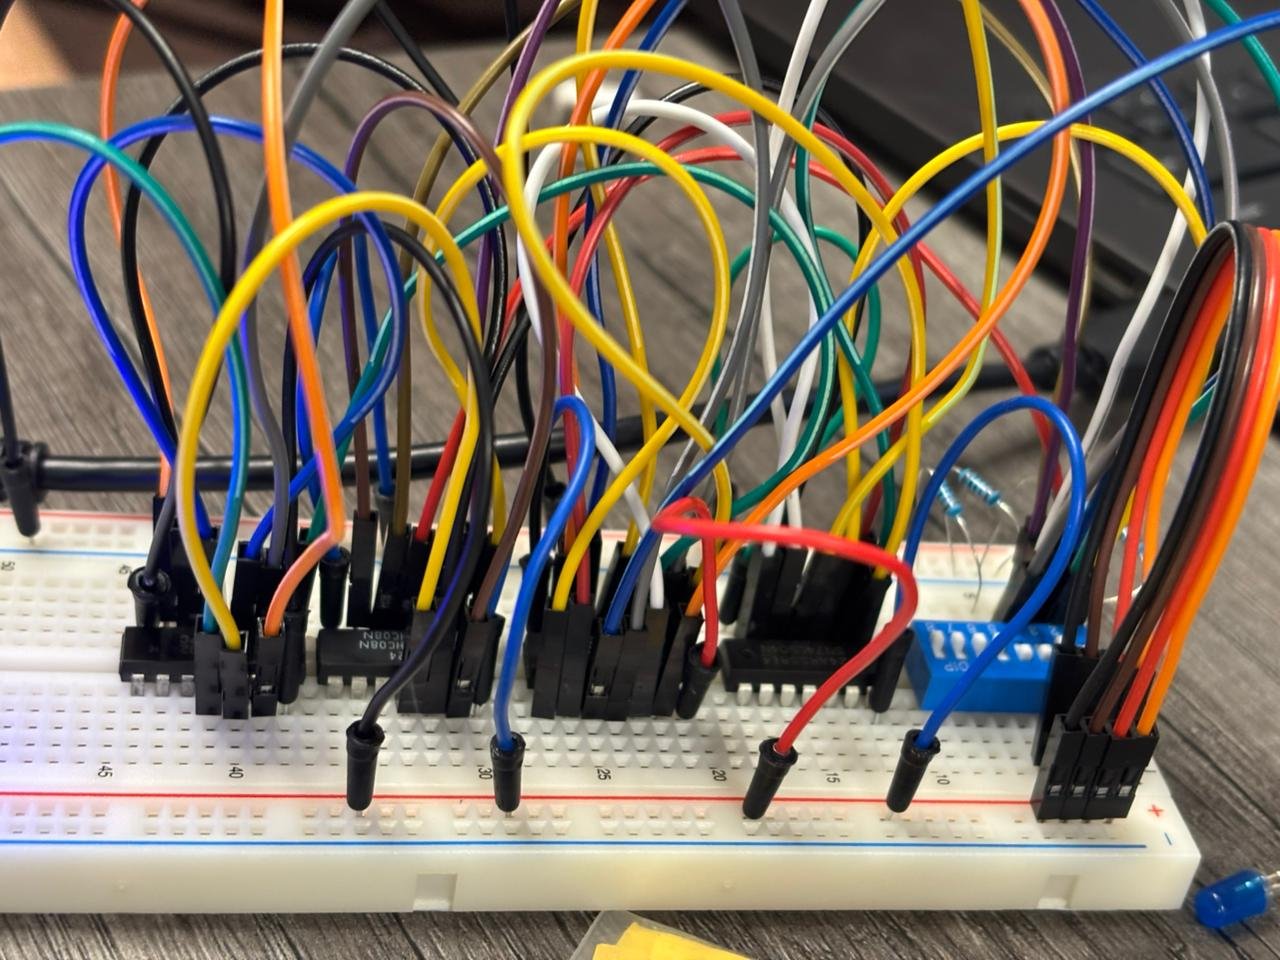
\includegraphics[width=0.4\textwidth]{Point5.jpg}
  \caption{Circuit built in breadboard simulating the Point 5 function.}
  \label{fig:circuit_point_5}
\end{figure}
\subsection{Digital lab experimentation}
After the development of the physical lab, the team developed in Multisim the same circuits developed in the physical lab, to properly organize and correct if necessary any errors.
In the first place, each logic gate was developed and tested:
\begin{figure}[H]
  \centering
  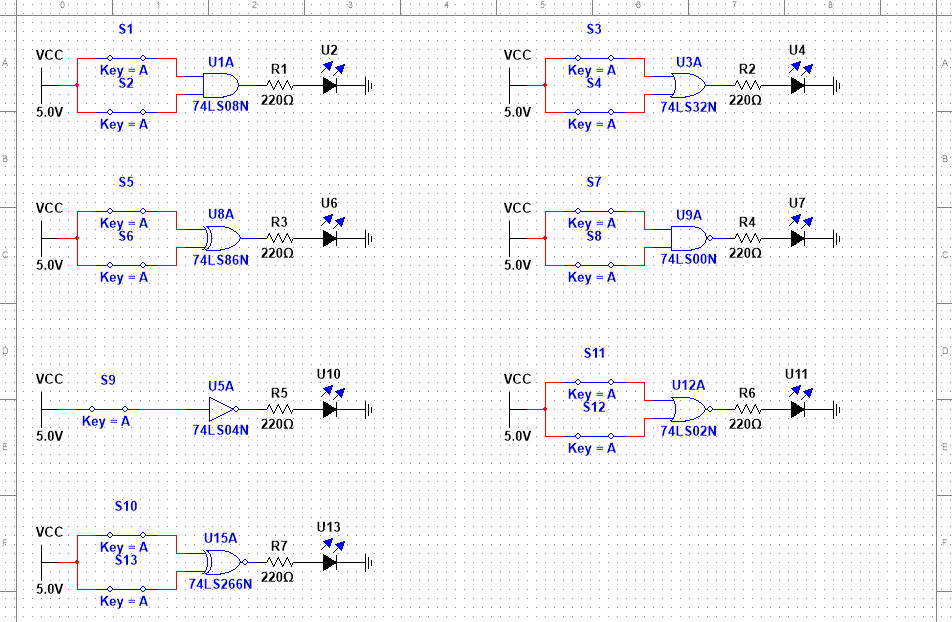
\includegraphics[width=0.4\textwidth]{LogiGates.png}
  \caption{Simulation of the Logic Gates}
  \label{fig:sim_logic_gates}
\end{figure}
And then, the point 5 circuit was designed in the plataform:
\begin{figure}[H]
  \centering
  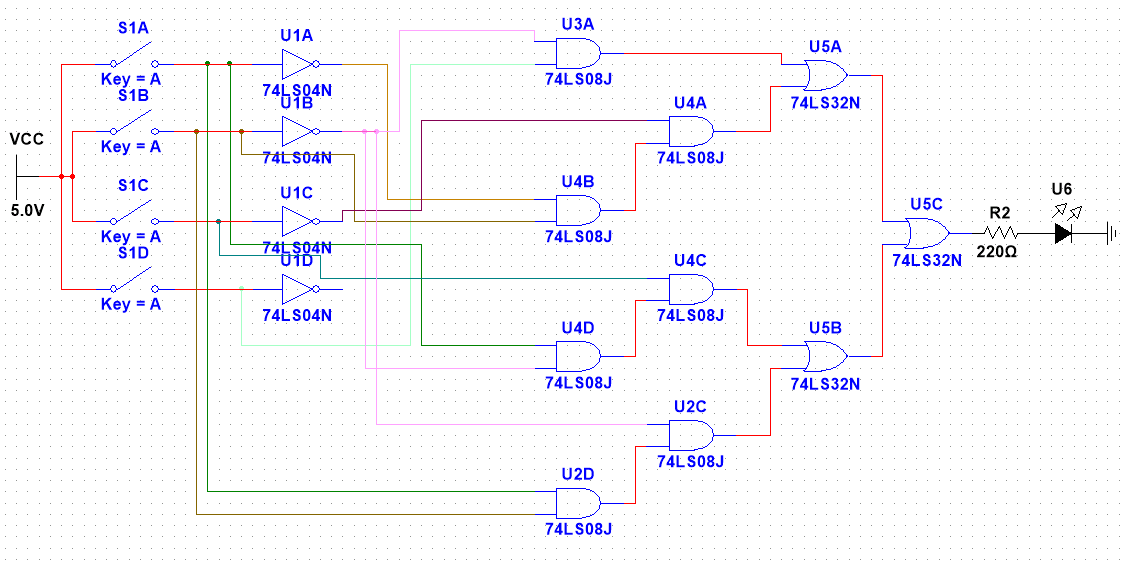
\includegraphics[width=0.4\textwidth]{Point5Multisim.png}
  \caption{Simulation of the point 5 funciton circuit}
  \label{fig:sim_point_5}
\end{figure}

\subsection{Codes}
Finally, the team developed codes in VHDL to prove the functionality of the circuits and function.
The first codes where developed in multiple files, one per logic gate:
\lstinputlisting[language=VHDL,caption=Code 1: AND gate]{codigos/AND.vhd}
\lstinputlisting[language=VHDL,caption=Code 2: OR gate]{codigos/OR.vhd}
\lstinputlisting[language=VHDL,caption=Code 3: NOT gate]{codigos/NOT.vhd}
\lstinputlisting[language=VHDL,caption=Code 4: NAND gate]{codigos/NAND.vhd}
\lstinputlisting[language=VHDL,caption=Code 5: NOR gate]{codigos/NOR.vhd}
\lstinputlisting[language=VHDL,caption=Code 6: XOR gate]{codigos/XOR.vhd}
\lstinputlisting[language=VHDL,caption=Code 7: XNOR gate]{codigos/XNOR.vhd}
After the development of these codes in EDA PLygrounds, the team created a code that showcases the boolean function of point 5:
\lstinputlisting[language=VHDL,caption=Code 8: Point 5 Code]{codigos/point5.vhd}
And to test this code, the team created the following:
\lstinputlisting[language=VHDL,caption=Code 1: Point 5 Testbench]{codigos/point5testbench.vhd}




\section{Analysis} %Análisis de los resultados obtenidos
Based on the data obtained during the laboratory practice, the observed behavior of the logic gates corresponds correctly to the expected truth tables. The discrepancies that initially appeared in the practical implementation were due to wiring errors and circuit organization, which were later corrected.
After completing the laboratory, the circuits were reproduced in Multisim to ensure proper organization and eliminate any possible mistakes. Each logic gate was tested individually, confirming its correct functionality. Finally, the circuits were implemented in EDA Playground using VHDL, where their behavior was simulated and verified. The results in this environment also matched the theoretical expectations, validating the practical and simulated work.
In conclusion, both the laboratory implementation and the digital simulations in Multisim and VHDL confirm the correct functionality of the logic gates and the designed circuits.
\section{Conclusions} %Conclusiones del reporte
The development of this practice made it possible to implement and verify the operation of three basic logic gates, both in the laboratory and in the simulation environments. The use of the multimeter was essential to confirm the correct functioning of the digital circuits, strengthening the understanding of measurement and verification processes in electronics.
Additionally, the Boolean function was analyzed by obtaining its truth table and canonical form, which was then implemented and validated experimentally. This analysis was complemented with simulations in Multisim and programming in VHDL through EDA Playground, confirming the correct logical behavior of the circuits and the function in different environments.
In this way, the proposed objectives were satisfactorily achieved, as the laboratory practice not only allowed the experimental validation of theoretical principles but also demonstrated the usefulness of digital simulation tools such as Multisim and VHDL for predicting and verifying circuit behavior.

%%%%%%% Bibliografía %%%%%%%%
\clearpage %Asegura que la bibliografía inicie en una nueva página
\bibliographystyle{bst/IEEEtran} %Estilo de bibliografía NO MODIFICAR PARA MANTENER FORMATO
\bibliography{bib/bibliografia} %Fuentes bibliográficas Se recomienda utilizar un gestor de referencias (zotero, jabref, etc..)
%%%%%%% Bibliografía %%%%%%%%      
\end{document} %Termina el documento
%% Known issues and TODO list%%%
% Warning overfull \hbox en los códigos
% Código en texto blanco y negro y comentarios en negritas => Cambiar a formato en colores